\chapter{L'interfaccia grafica}\label{cap:interfaccia}

L'interfaccia grafica del programma, oltre a offrire la possibilità di azionare e mettere in pausa l'accordatore, permette di selezionare la modalità con cui definire la frequenza di riferimento, mostra la nota corrispondente a tale frequenza e visualizza la distanza tra la frequenza del suono in input e il valore di riferimento.

È possibile, infatti, indicare esplicitamente la nota da prendere come riferimento oppure lasciar riconoscere all'accordatore tale frequenza in modalità automatica.
Questa seconda opzione risulta comoda quando le corde della chitarra sono leggermente fuori tonalità.
In questo caso, infatti, il software riconosce facilmente la frequenza di riferimento senza la necessità che l'utente debba impostarne il valore manualmente.

	\begin{figure}[h]
	  \begin{center} 
	    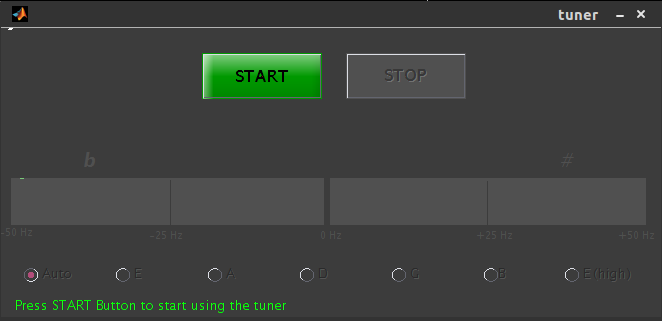
\includegraphics[width=\textwidth*\real{0.8}]{images/ch_07/accordatore_fermo.png}
	  \end{center} 
	  \caption{\textit{Accordatore pronto per essere avviato}}  
	  \label{fig:accordatore_fermo}
	\end{figure}

La figura \ref{fig:accordatore_fermo} mostra la visione che ha l'utente nel momento in cui avvia il programma.
L'accordatore è spento, per azionarlo è necessario premere il bottone \emph{Start}, come suggerisce il messaggio nell'angolo in basso a sinistra della finestra.

Al momento dell'avvio, una serie di operazioni vengono eseguite.
Innanzitutto, viene attivato il timer che regola il funzionamento dell'accordatore.
In secondo luogo, il software avvia la registrazione.
Infine, l'interfaccia grafica viene modificata in modo tale da permettere all'utente di usufruire delle funzionalità del software.

Il timer ha la funzione di chiamare la funzione di tuning una volta al secondo. 
Tale funzione effettua le seguenti operazioni:
\begin{itemize}
	\item fermare il registratore,
	\item estrarre i dati registrati dal buffer del registratore,
	\item riattivare il registratore,
	\item chiamare la procedura di riconoscimento delle frequenza del suono in ingresso,
	\item calcolare la distanza tra frequenza del suono in input e frequenza di riferimento,
	\item aggiornare l'interfaccia grafica con i dati appena calcolati.
\end{itemize}

L'utente ha la possibilità di cambiare la frequenza di riferimento grazie ai bottoni che si trovano nella parte bassa della finestra, appena al di sopra del messaggio di aiuto.

	\begin{figure}[h]
	  \begin{center} 
	    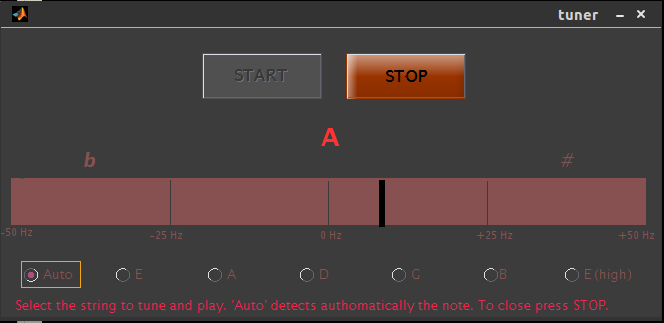
\includegraphics[width=\textwidth*\real{0.8}]{images/ch_07/accordatore_auto.png}
	  \end{center} 
	  \caption{\textit{Accordatore in funzione in modalità automatica}}  
	  \label{fig:accordatore_in_funzione}
	\end{figure}

L'aggiornamento dell'interfaccia consiste nel mostrare la nota di riferimento al di sotto dei bottoni \emph{Start} e \emph{Stop} e nel muovere l'indicatore nero lungo la barra delle frequenze in funzione della distanza misurata tra il suono in input e quello di riferimento. 
In figura \ref{fig:accordatore_in_funzione}, si può vedere l'accordatore, in modalità automatica, mentre fornisce la distanza tra la frequenza della nota in ingresso e la nota di riferimento che, in questo caso, è un LA.



